\subsection{ Mô hình hóa tương tác}
\subsubsection{Use case diagram}

\subsubsection*{Application Use Case}
\begin{figure}[H]
    \centering
    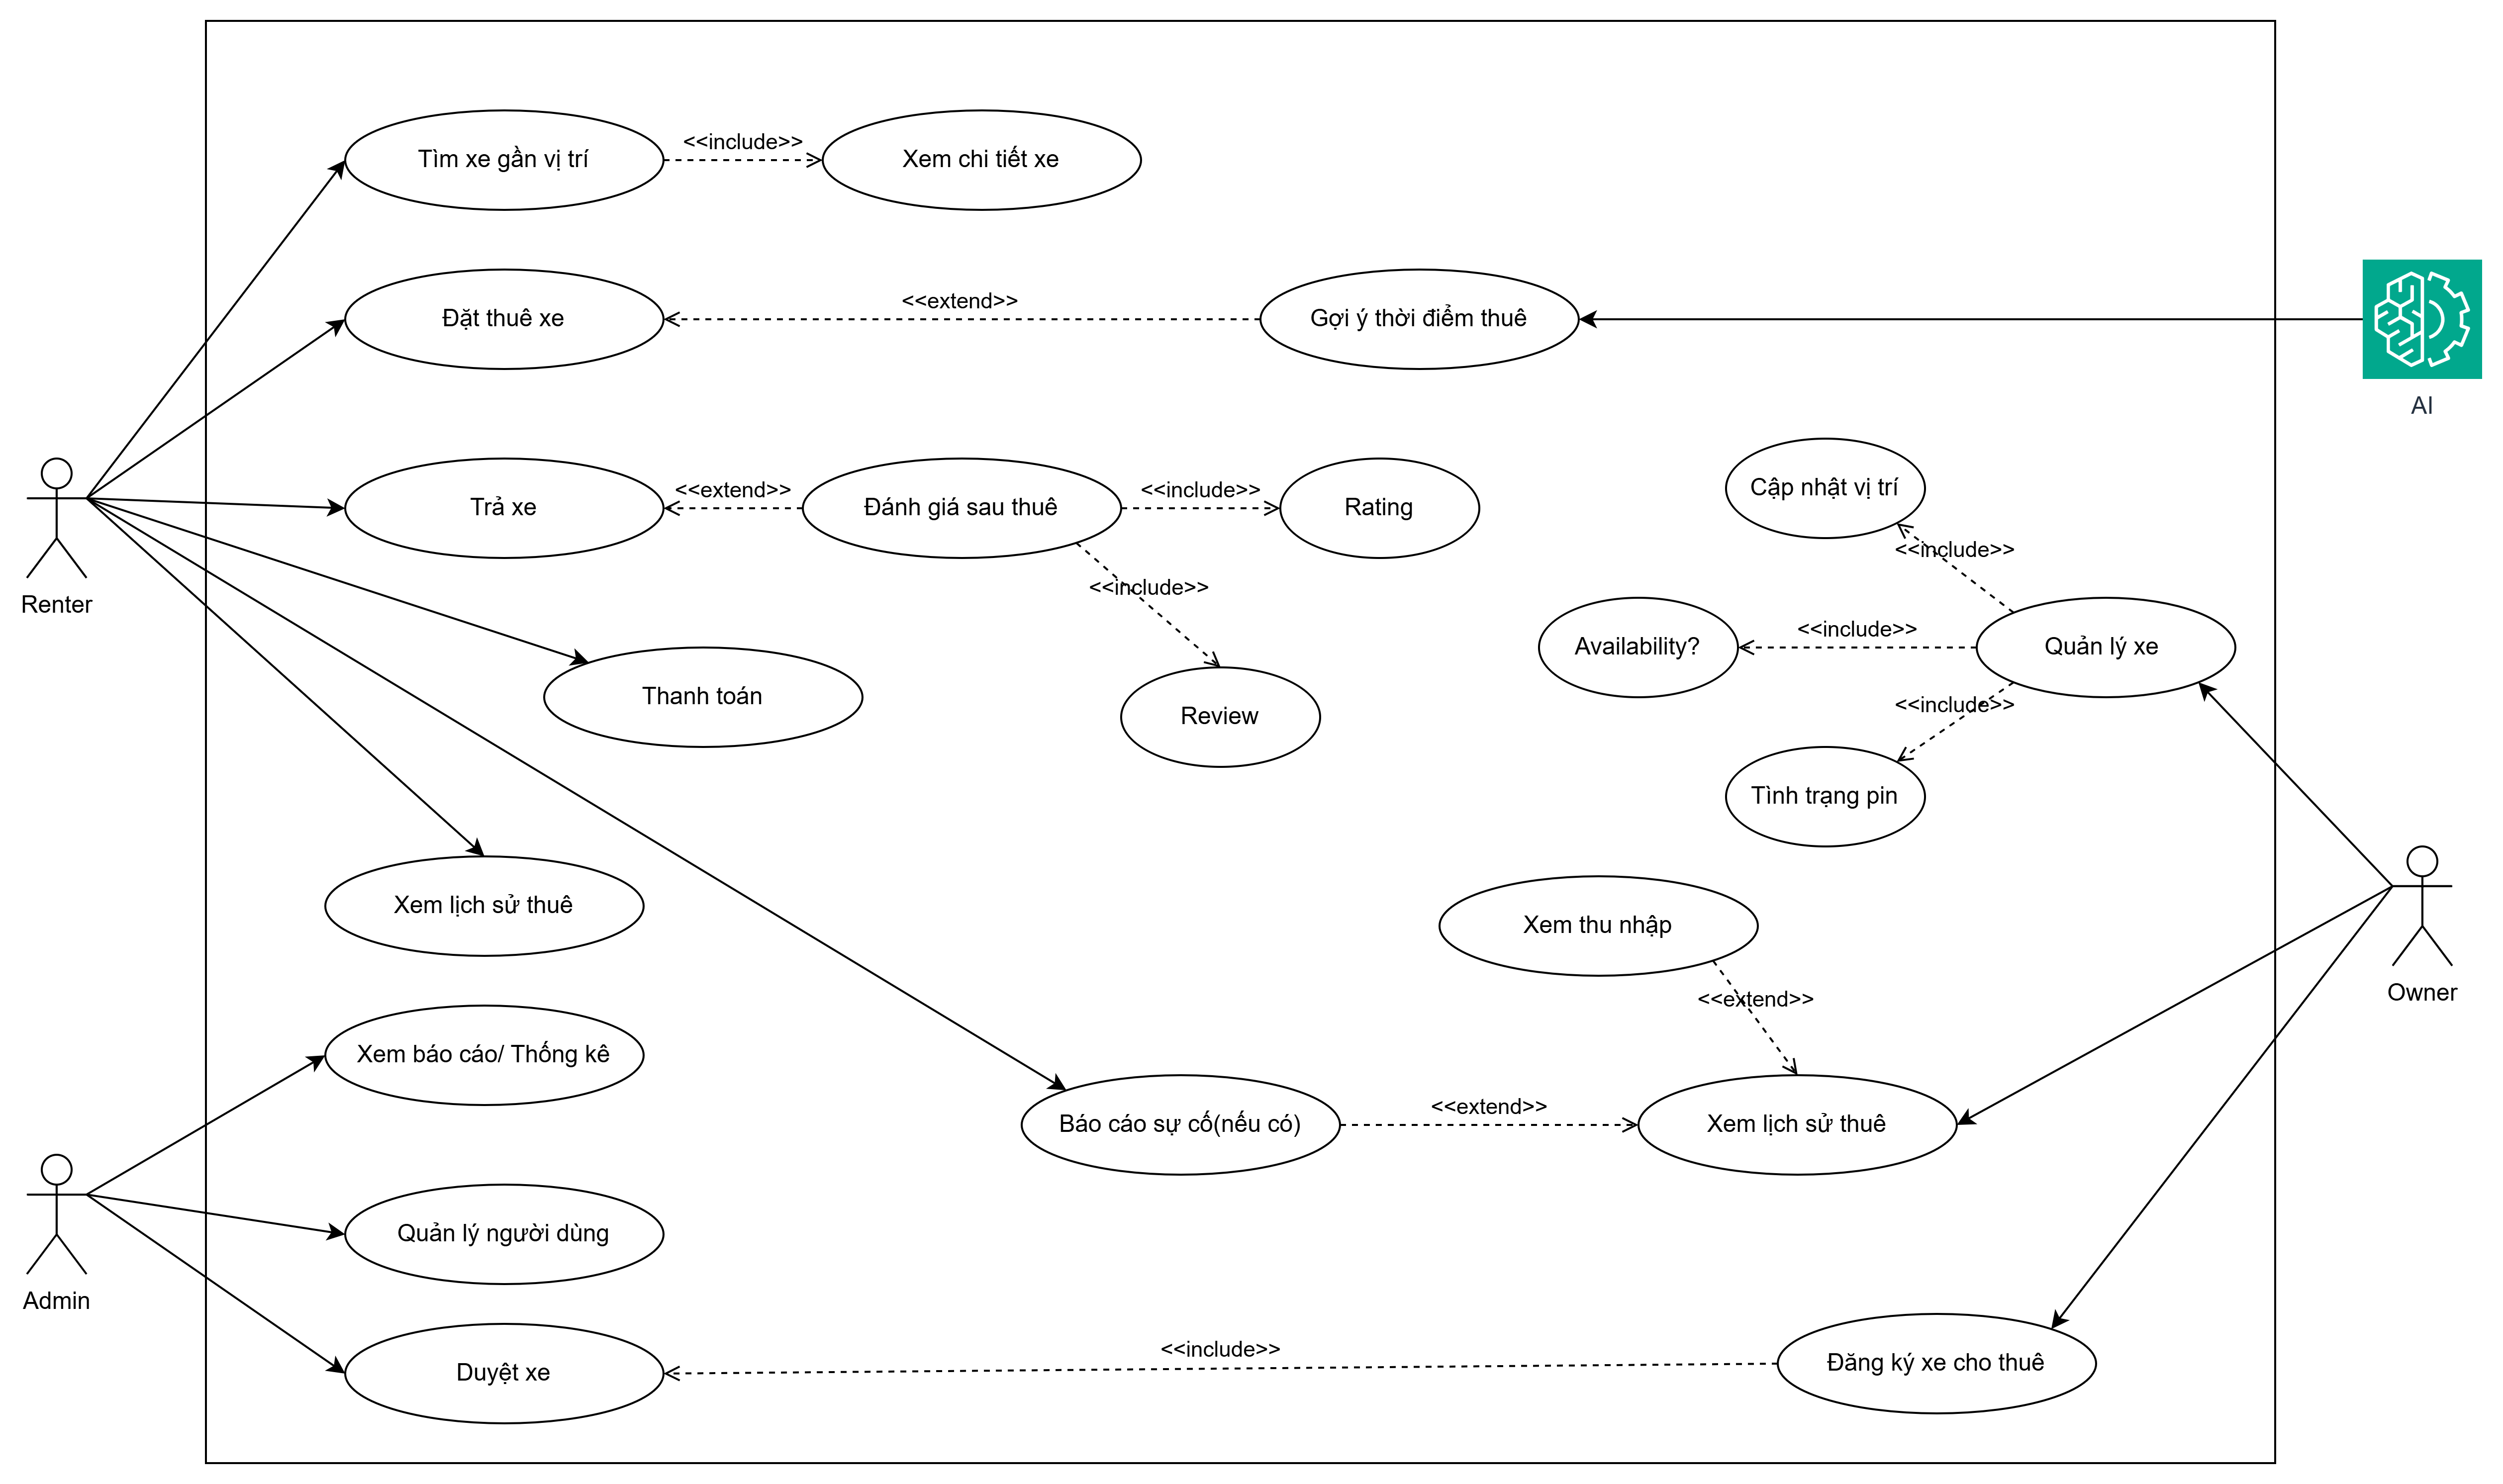
\includegraphics[width=1\textwidth]{Images/Usecase/system.png}
    \caption{Application Use Case Diagram}
\end{figure}

\begin{itemize}
    \item \textbf{UC-01:} Đăng ký / Đăng nhập
    \item \textbf{UC-13:} Đánh giá \& Xếp hạng người dùng (Trust Score System)
    \item \textbf{UC-14:} Gợi ý thời điểm thuê (Recommendation)
    \item \textbf{UC-15:} Xem lịch sử thuê / thu nhập (của Owner hoặc Renter)
    \item \textbf{UC-16:} Báo cáo sự cố (Renter/Owner)
    \item \textbf{UC-17:} Thông báo
    \item \textbf{Renter Use Case}
    \item \textbf{Owner Use Case}
    \item \textbf{Admin Use Case}
\end{itemize}

\vspace{0.5cm}
\subsubsection*{Renter Use Case}
\begin{itemize}
    \item \textbf{UC-02:} Tìm xe gần vị trí
    \item \textbf{UC-03:} Xem chi tiết xe
    \item \textbf{UC-04:} Đặt thuê xe
    \item \textbf{UC-05:} Trả xe
    \item \textbf{UC-06:} Thanh toán
    \item \textbf{UC-07:} Đánh giá sau thuê (Rating / Review)
\end{itemize}
\begin{figure}[H]
    \centering
    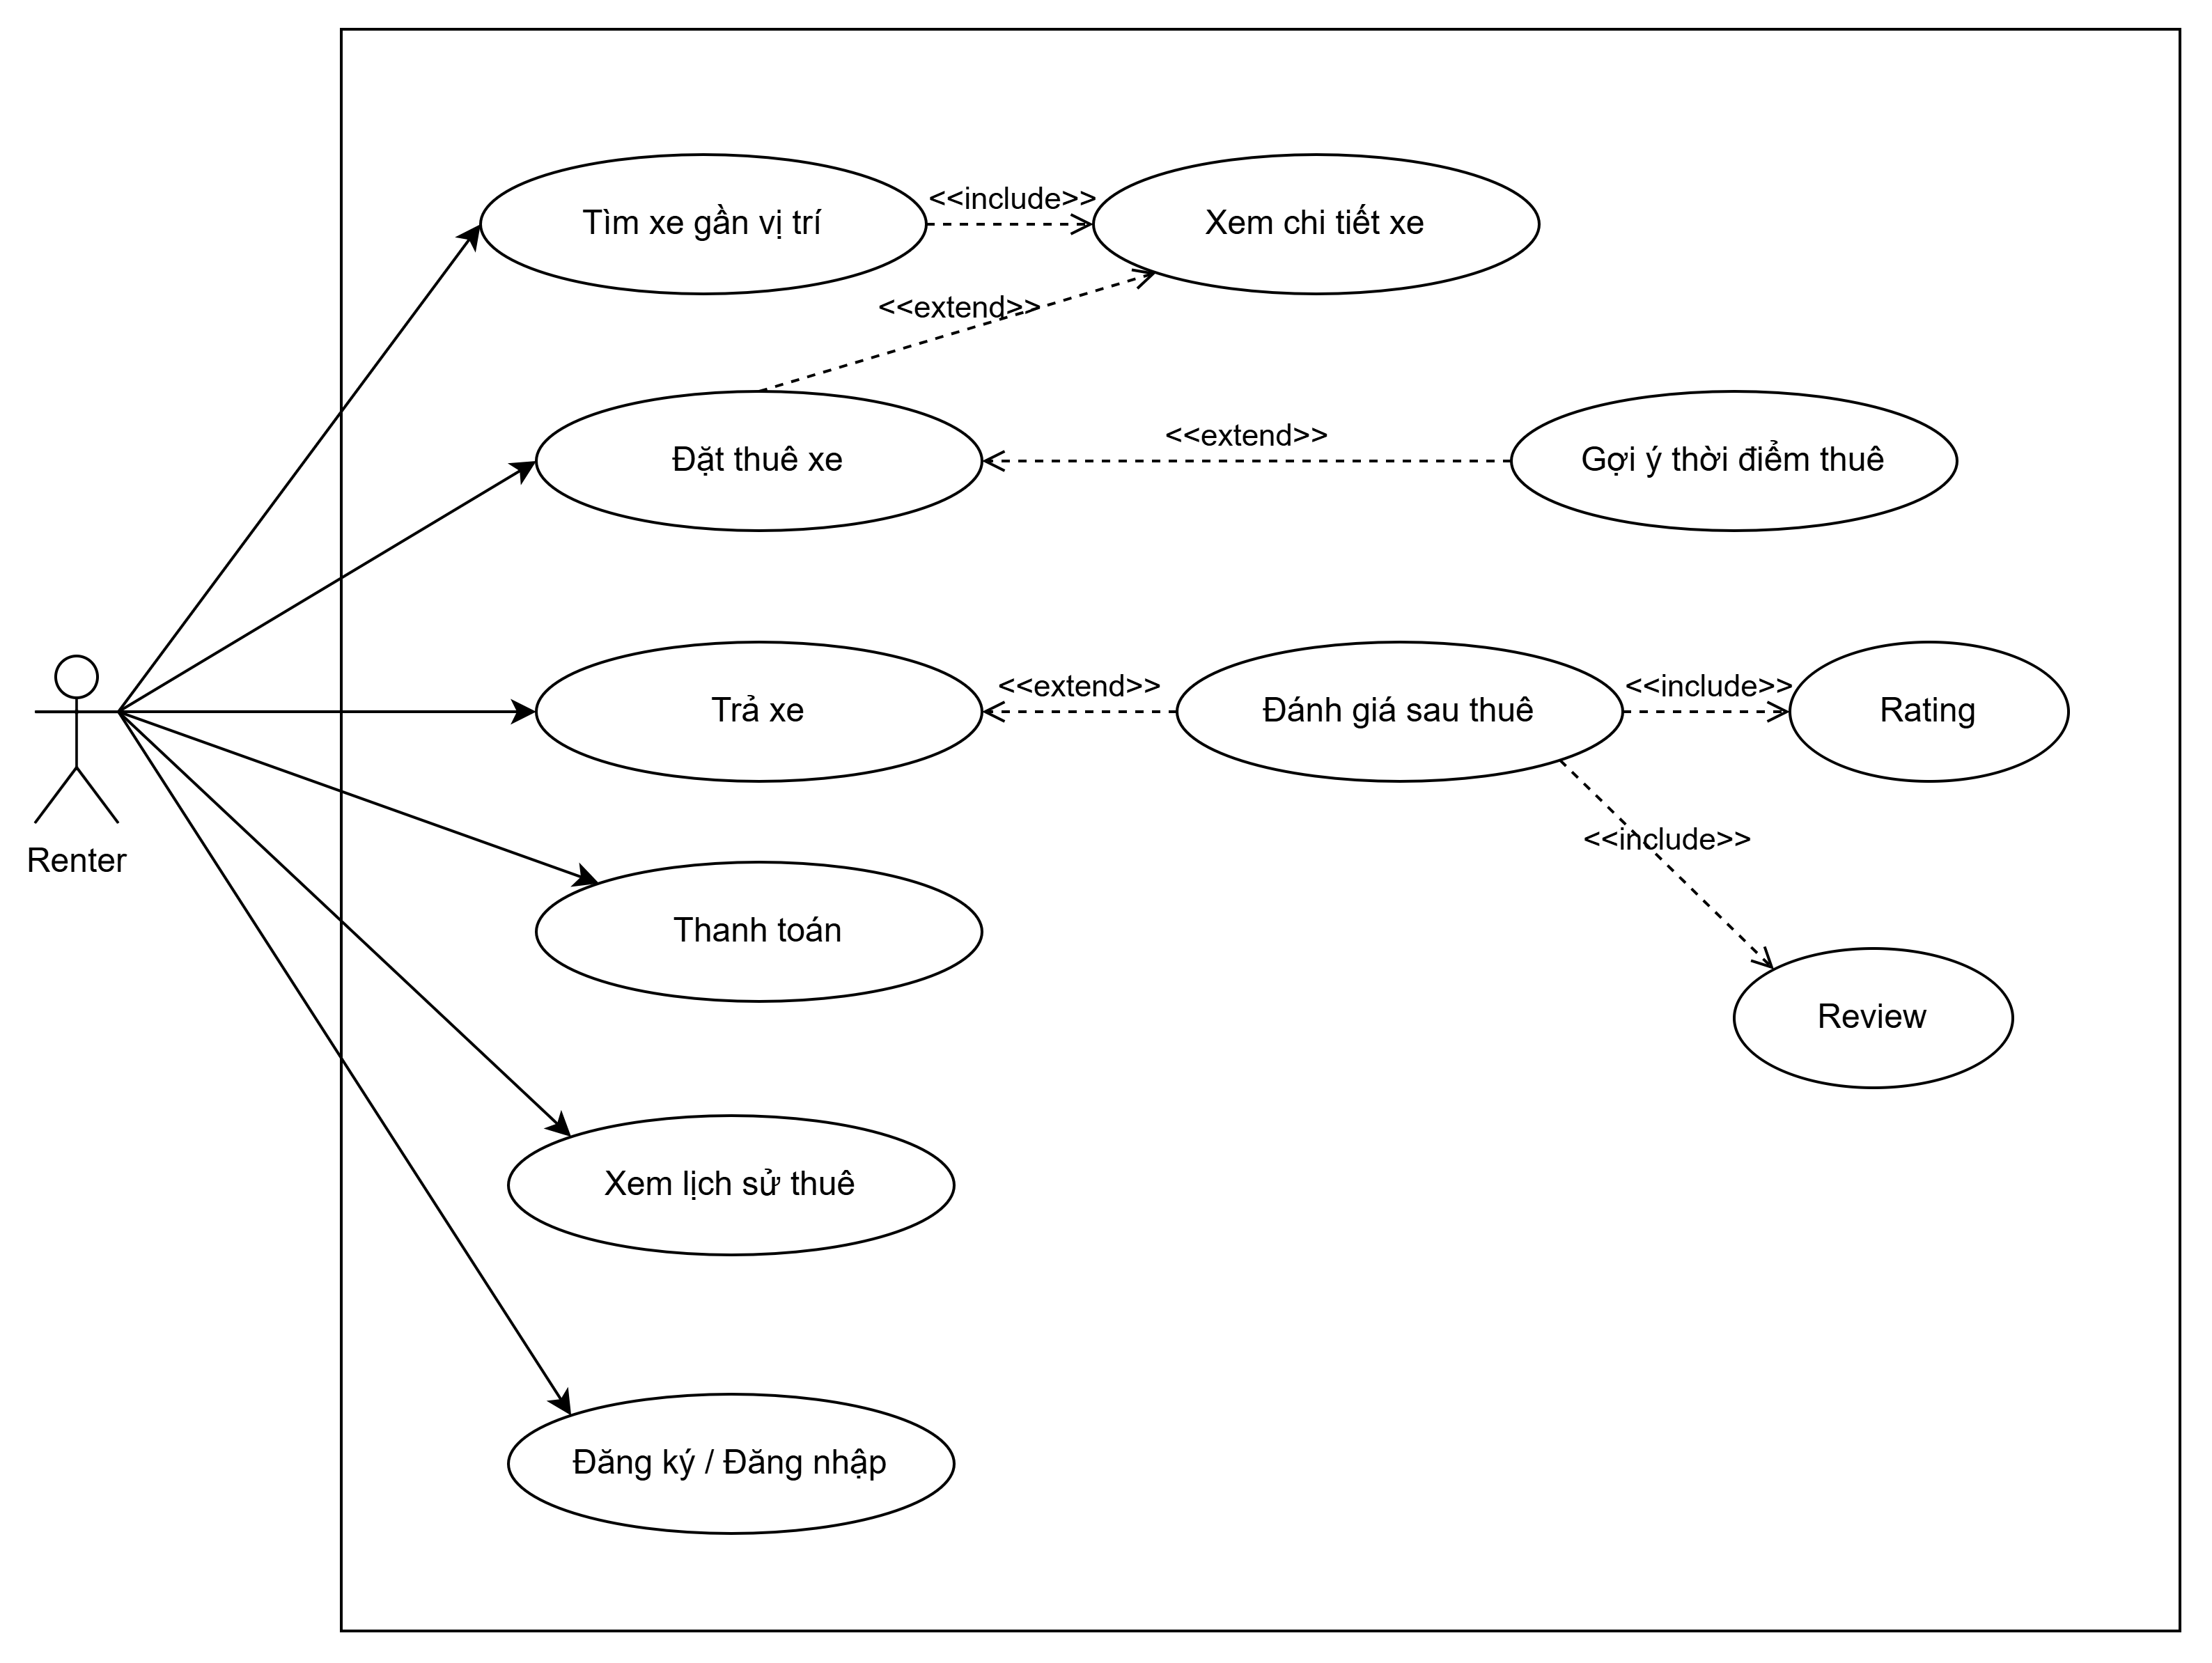
\includegraphics[width=0.85\textwidth]{Images/Usecase/renter.png}
    \caption{Renter Use Case Diagram}
\end{figure}

\subsubsection*{Owner Use Case}
\begin{itemize}
    \item \textbf{UC-08:} Đăng ký xe cho thuê (Owner)
    \item \textbf{UC-09:} Quản lý xe (Owner quản lý availability, cập nhật vị trí, pin)
\end{itemize}
\begin{figure}[H]
    \centering
    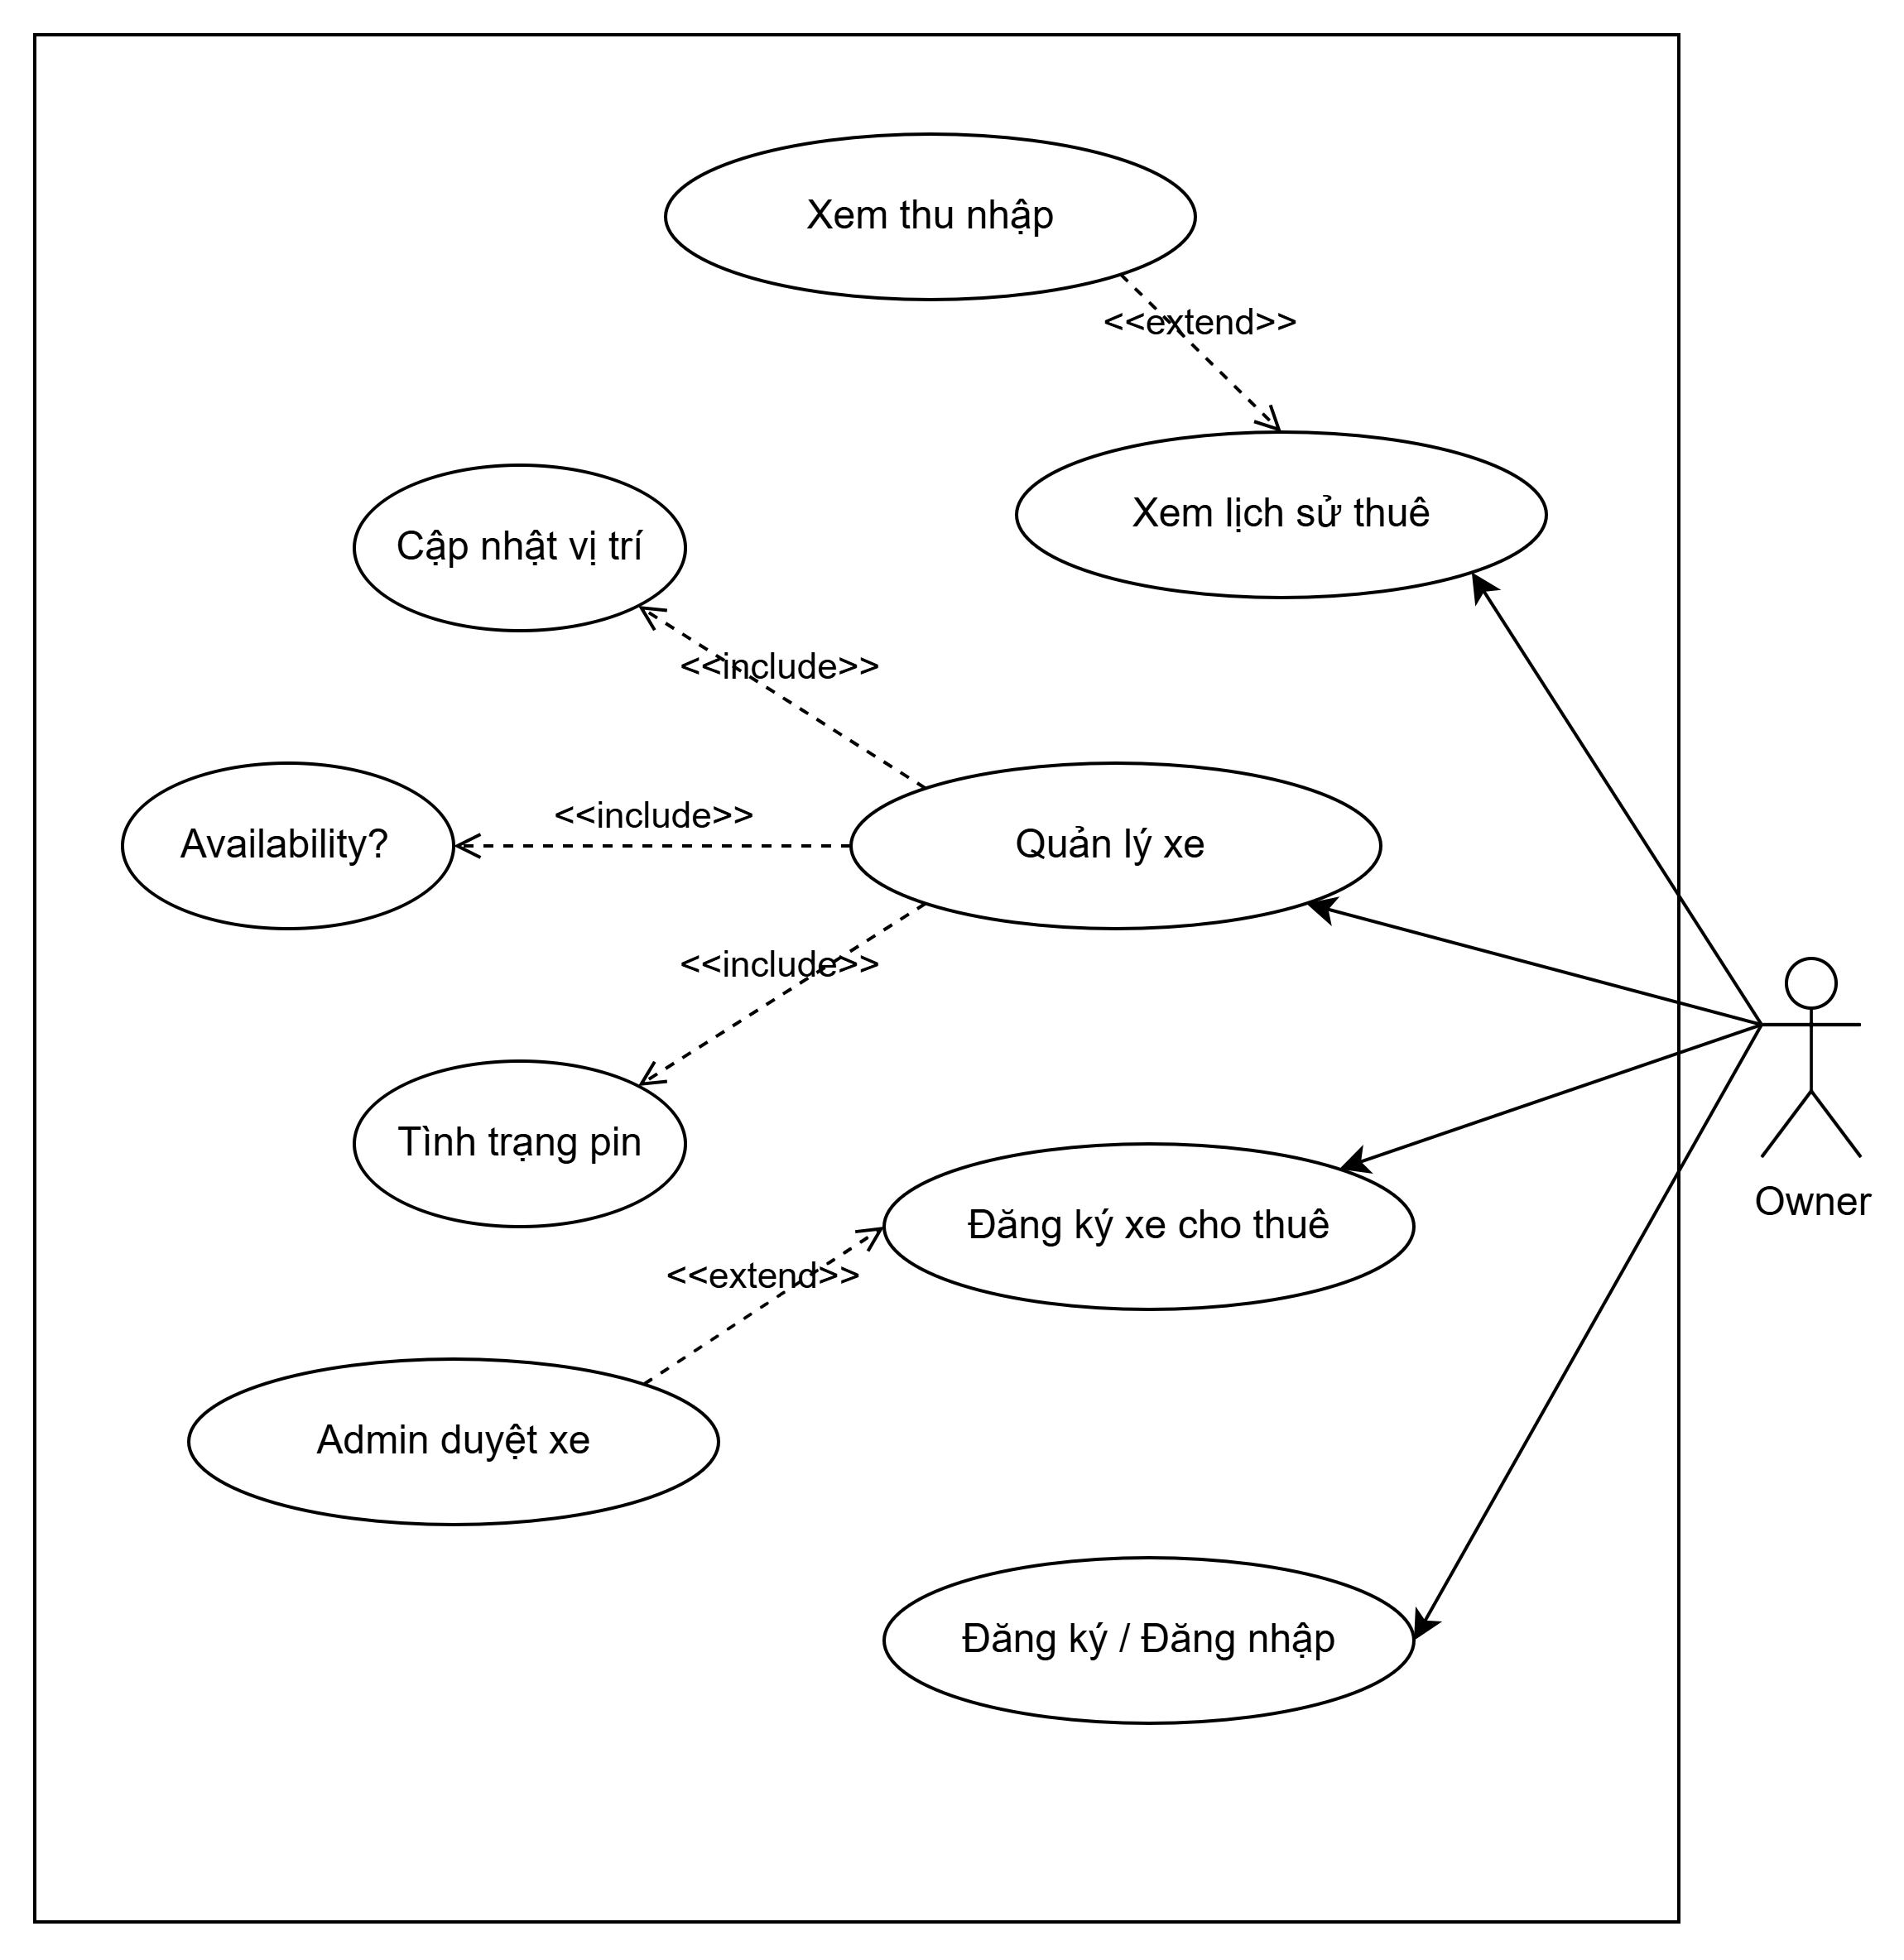
\includegraphics[width=0.65\textwidth]{Images/Usecase/owner.png}
    \caption{Owner Use Case Diagram}
\end{figure}

\subsubsection*{Admin Use Case}
\begin{figure}[H]
    \centering
    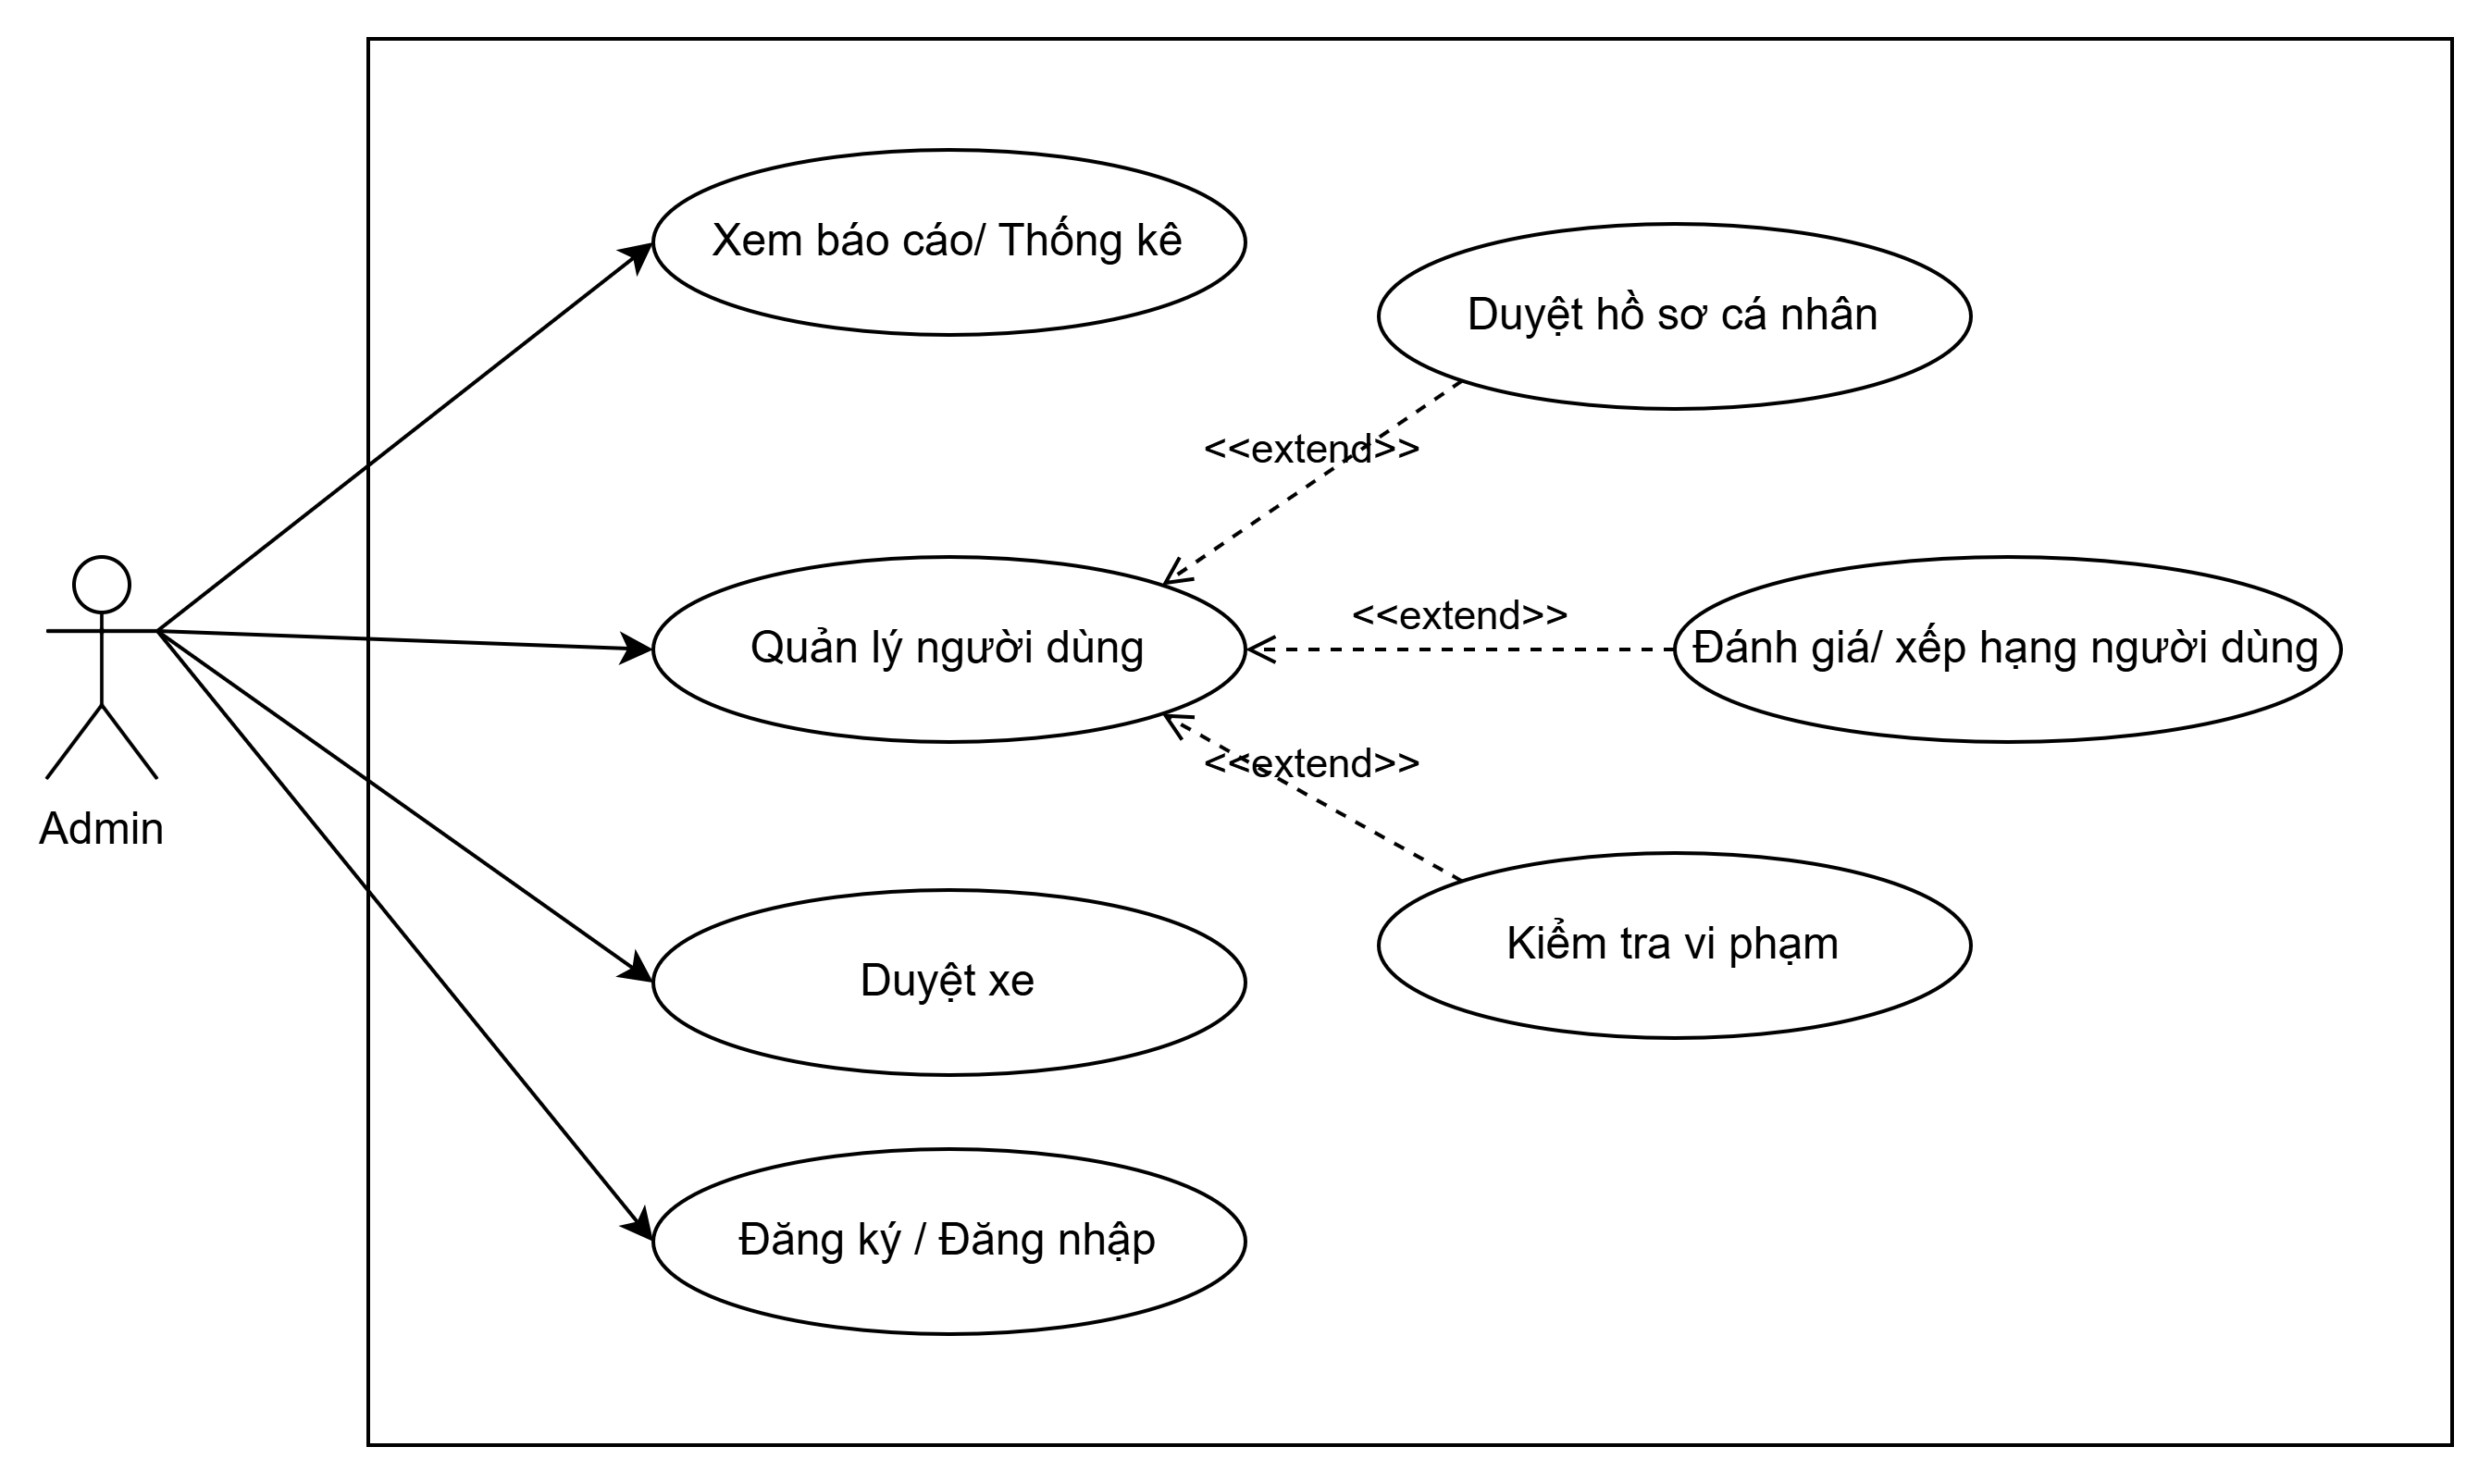
\includegraphics[width=0.65\textwidth]{Images/Usecase/admin.png}
    \caption{Admin Use Case Diagram}
\end{figure}

\begin{itemize}
    \item \textbf{UC-10:} Duyệt xe / Quản trị hệ thống (Admin)
    \item \textbf{UC-11:} Xem báo cáo / Thống kê (Admin)
    \item \textbf{UC-12:} Quản lý người dùng
\end{itemize}

\subsubsection{Use case description}

\subsubsection*{UC-01 –Đăng ký / Đăng nhập}

\begin{longtable}{|>{\raggedright\arraybackslash}p{4cm}|>{\raggedright\arraybackslash}p{11cm}|}
\hline
\textbf{Trường} & \textbf{Mô tả} \\
\hline
\endfirsthead

\hline
\textbf{Trường} & \textbf{Mô tả} \\
\hline
\endhead

\hline
\endfoot

Actor & Người dùng (Customer / Vehicle Owner / Admin) \\
\hline
Description & Người dùng đăng ký tài khoản mới hoặc đăng nhập vào hệ thống. \\
\hline
Trigger & Người dùng chọn "Đăng ký / Đăng nhập" trên giao diện. \\
\hline
Precondition & Ứng dụng hoạt động, có kết nối mạng. \\
\hline
Postcondition & Người dùng được xác thực và truy cập vào giao diện cá nhân. \\
\hline
Normal Flow & 1. Người dùng nhập email/số điện thoại và mật khẩu. \newline 2. Hệ thống kiểm tra thông tin. \newline 3. Nếu hợp lệ, đăng nhập thành công. \newline 4. Chuyển hướng tới màn hình chính. \\
\hline
Alt Flow & A1. Người dùng chọn "Quên mật khẩu" → Hệ thống gửi OTP khôi phục. \newline A2. Người dùng chọn "Đăng ký" → điền thông tin, gửi yêu cầu xác thực. \\
\hline
Exception Flow & E1. Sai mật khẩu quá 5 lần → tạm khóa tài khoản. \newline E2. Hệ thống lỗi kết nối → hiển thị thông báo "Không thể đăng nhập, vui lòng thử lại." \\
\hline
\end{longtable}

\subsubsection*{UC-02 – Tìm xe gần vị trí}

\begin{longtable}{|>{\raggedright\arraybackslash}p{4cm}|>{\raggedright\arraybackslash}p{11cm}|}
\hline
\textbf{Trường} & \textbf{Mô tả} \\
\hline
\endfirsthead

\hline
\textbf{Trường} & \textbf{Mô tả} \\
\hline
\endhead

\hline
\endfoot

\textbf{Tên Use Case} & Tìm xe gần vị trí \\
\hline
\textbf{Actor chính} & Người thuê xe (Renter) \\
\hline
\textbf{Mục tiêu} & Giúp người dùng tìm xe khả dụng trong khu vực xung quanh, dựa trên \textbf{vị trí hiện tại (GPS)} hoặc \textbf{vị trí nhập tay} để đặt trước. \\
\hline
\textbf{Trigger} & Người dùng nhấn ``Tìm xe gần tôi'' hoặc chọn ``Nhập vị trí khác''. \\
\hline
\textbf{Precondition} & Người dùng đã đăng nhập; có quyền truy cập bản đồ; GPS được bật hoặc người dùng nhập vị trí thủ công. \\
\hline
\textbf{Postcondition} & Danh sách xe khả dụng được hiển thị theo khu vực được chọn. \\
\hline
\textbf{Normal Flow} & 
1. Người dùng chọn ``Tìm xe gần tôi''. \newline
2. Hệ thống yêu cầu quyền truy cập vị trí GPS. \newline
3. Ứng dụng lấy vị trí hiện tại của người dùng. \newline
4. Backend truy vấn danh sách xe khả dụng trong bán kính. \newline
5. Hệ thống hiển thị các xe gần nhất cùng thông tin: khoảng cách, mức pin, giá thuê, đánh giá. \newline
6. Người dùng chọn một xe để xem chi tiết. \\
\hline
\textbf{Alt Flow} & 
1. Người dùng chọn ``Nhập vị trí khác''. \newline
2. Hệ thống hiển thị hộp tìm kiếm địa điểm. \newline
3. Người dùng nhập địa chỉ hoặc khu vực mong muốn. \newline
4. Hệ thống sử dụng Geocoding API để lấy tọa độ (lat, lng). \newline
5. Backend truy vấn danh sách xe khả dụng quanh vị trí đó. \newline
5.1. Nếu có xe khả dụng, hiển thị danh sách. \newline
5.2. Nếu không có xe, gợi ý mở rộng bán kính hoặc chọn thời gian khác.\\
\hline
\textbf{Exception Flow} & 
E1. Không có xe khả dụng → hiển thị thông báo ``Không có xe trong khu vực này.'' \newline
E2. GPS bị tắt và người dùng không nhập vị trí → yêu cầu bật định vị hoặc nhập vị trí thủ công. \newline
E3. Lỗi kết nối mạng → hiển thị thông báo ``Không thể tải dữ liệu. Vui lòng thử lại.'' \\
\hline
\textbf{Included Use Cases} & \texttt{UC-03 -- Xem chi tiết xe} \\
\hline
\textbf{Extended Use Cases} & \texttt{UC-04 -- Đặt thuê xe (Pre-booking)} \\
\hline
\textbf{Business Rules} &
- Vị trí nhập tay phải nằm trong khu vực hoạt động của hệ thống. \newline
- Với khoảng cách > 10km, hệ thống gợi ý chuyển sang khu vực gần hơn hoặc chế độ giao xe (nếu có). \newline
- Khi ``Đặt trước'', chỉ hiển thị xe có trạng thái \texttt{available} trong khung thời gian đã chọn. \\
\hline
\end{longtable}

\subsubsection*{UC-03 – Xem chi tiết xe}

\begin{longtable}{|>{\raggedright\arraybackslash}p{4cm}|>{\raggedright\arraybackslash}p{11cm}|}
\hline
\textbf{Trường} & \textbf{Mô tả} \\
\hline
\endfirsthead

\hline
\textbf{Trường} & \textbf{Mô tả} \\
\hline
\endhead

\hline
\endfoot

% Use Case ID & UC-03 \\
% \hline
Actor & Người thuê (Renter), Chủ xe (Owner) \\
\hline
Mục tiêu & Cho phép người dùng xem thông tin chi tiết của xe, bao gồm tình trạng pin, vị trí, giá thuê, đánh giá và thông tin chủ xe. \\
\hline
Trigger & Người dùng chọn một xe từ danh sách hiển thị (từ UC-02: "Tìm xe gần vị trí"). \\
\hline
Precondition & Xe tồn tại và đang ở trạng thái "có sẵn (available)". \\
\hline
Postcondition & Thông tin chi tiết hiển thị cho người dùng. \\
\hline
Normal Flow & 1. Người thuê chọn xe từ bản đồ hoặc danh sách. \newline 2. Server trả thông tin: hình ảnh, loại xe, tình trạng pin, vị trí hiện tại, giá, đánh giá trung bình, chủ xe. \newline 3. Ứng dụng hiển thị giao diện chi tiết xe. \newline 4. Người thuê có thể chọn "Đặt thuê xe" \\
\hline
Alternative Flow & A1. Người thuê thêm xe vào danh sách "Yêu thích" (wishlist). \newline A2. Người thuê chia sẻ đường dẫn xe cho người khác (social sharing). \\
\hline
Exception Flow & E1. Xe đã bị ẩn hoặc đang thuê → hiển thị thông báo "Xe không khả dụng". \newline E2. Lỗi tải dữ liệu → hiển thị "Không thể tải thông tin xe". \\
\hline
Included Use Cases & \texttt{Xem đánh giá (Review)} \\
\hline
Extended Use Cases & \texttt{Đặt thuê xe (UC-04)} \\
\hline
\end{longtable}

\subsubsection*{UC-04 – Đặt thuê xe}

\begin{longtable}{|>{\raggedright\arraybackslash}p{4cm}|>{\raggedright\arraybackslash}p{11cm}|}
\hline
\textbf{Trường} & \textbf{Mô tả} \\
\hline
\endfirsthead

\hline
\textbf{Trường} & \textbf{Mô tả} \\
\hline
\endhead

\hline
\endfoot

Actor & Người thuê xe \\
\hline
Description & Đặt trước xe để thuê trong khoảng thời gian mong muốn. \\
\hline
Trigger & Người dùng nhấn "Đặt thuê" trên chi tiết xe. \\
\hline
Precondition & Xe đang ở trạng thái "Available", người dùng đã đăng nhập. \\
\hline
Postcondition & Đơn đặt xe được ghi nhận và chờ xác nhận. \\
\hline
Normal Flow & 1. Người dùng chọn thời gian thuê. \newline 2. Hệ thống gợi ý thời điểm thuê tối ưu (AI). \newline 3. Người dùng xác nhận đặt thuê. \newline 4. Hệ thống tạo đơn và gửi thông báo cho chủ xe. \\
\hline
Alt Flow & A1. Người thuê thay đổi thời gian thuê → hệ thống cập nhật chi phí tương ứng. \newline A2. Chủ xe từ chối yêu cầu thuê. \\
\hline
Exception Flow & E1. Xe đã được người khác đặt trước → hiển thị thông báo lỗi. \newline E2. Lỗi thanh toán hoặc xác nhận mạng. \\
\hline
Extended Use Cases & \texttt{Gợi ý thời điểm thuê} \\
\hline
\end{longtable}

\subsubsection*{UC-05 – Trả xe}

\begin{longtable}{|>{\raggedright\arraybackslash}p{4cm}|>{\raggedright\arraybackslash}p{11cm}|}
\hline
\textbf{Trường} & \textbf{Mô tả} \\
\hline
\endfirsthead

\hline
\textbf{Trường} & \textbf{Mô tả} \\
\hline
\endhead

\hline
\endfoot

Actor & Người thuê xe \\
\hline
Description & Người thuê kết thúc hành trình và trả xe. \\
\hline
Trigger & Người thuê chọn "Trả xe" trên giao diện. \\
\hline
Precondition & Xe đang trong trạng thái thuê. \\
\hline
Postcondition & Xe được cập nhật trạng thái "Available". \\
\hline
Normal Flow & 1. Người thuê xác nhận trả xe. \newline 2. Hệ thống cập nhật vị trí trả xe và tính tổng chi phí. \newline 3. Thanh toán hoàn tất. \newline 4. Hiển thị màn hình đánh giá. \\
\hline
Alt Flow & A1. Người thuê trả xe sớm hơn dự kiến → hệ thống điều chỉnh chi phí. \\
\hline
Exception Flow & E1. Không thể xác định vị trí xe → yêu cầu nhập vị trí thủ công. \newline E2. Lỗi hệ thống thanh toán. \\
\hline
Extended Use Cases & \texttt{Đánh giá sau thuê} \\
\hline
\end{longtable}

\subsubsection*{UC-06 – Thanh toán}

\begin{longtable}{|>{\raggedright\arraybackslash}p{4cm}|>{\raggedright\arraybackslash}p{11cm}|}
\hline
\textbf{Trường} & \textbf{Mô tả} \\
\hline
\endfirsthead

\hline
\textbf{Trường} & \textbf{Mô tả} \\
\hline
\endhead

\hline
\endfoot

Actor & Người thuê xe \\
\hline
Description & Thực hiện thanh toán sau khi hoàn tất thuê xe hoặc đặt cọc trước khi thuê. \\
\hline
Trigger & Khi người dùng hoàn tất hành trình hoặc xác nhận đặt thuê. \\
\hline
Precondition & Người dùng đã chọn phương thức thanh toán (thẻ, ví điện tử, v.v.). \\
\hline
Postcondition & Giao dịch thanh toán thành công, lưu thông tin hóa đơn. \\
\hline
Normal Flow & 1. Hệ thống tính toán chi phí thuê (thời gian × giá). \newline 2. Hiển thị tổng tiền và yêu cầu xác nhận thanh toán. \newline 3. Người dùng xác nhận. \newline 4. Hệ thống kết nối cổng thanh toán (mock/payment gateway). \newline 5. Trạng thái cập nhật thành "Paid". \\
\hline
Alt Flow & A1. Người thuê chọn thanh toán bằng điểm thưởng hoặc ví điện tử nội bộ. \newline A2. Thanh toán tự động qua thẻ lưu sẵn. \\
\hline
Exception Flow & E1. Giao dịch thất bại → hoàn tác đặt xe. \newline E2. Cổng thanh toán không phản hồi → thông báo "Thử lại sau". \\
\hline
\end{longtable}

\subsubsection*{UC-07 – Đánh giá sau thuê}

\begin{longtable}{|>{\raggedright\arraybackslash}p{4cm}|>{\raggedright\arraybackslash}p{11cm}|}
\hline
\textbf{Trường} & \textbf{Mô tả} \\
\hline
\endfirsthead

\hline
\textbf{Trường} & \textbf{Mô tả} \\
\hline
\endhead

\hline
\endfoot

Actor & Người thuê xe \\
\hline
Description & Người dùng để lại đánh giá và chấm sao cho xe/chủ xe. \\
\hline
Trigger & Sau khi trả xe hoặc từ trang "Lịch sử thuê". \\
\hline
Precondition & Đã hoàn tất thuê xe. \\
\hline
Postcondition & Đánh giá được lưu trữ và cập nhật điểm trung bình. \\
\hline
Normal Flow & 1. Người dùng chọn số sao (1--5). \newline 2. Nhập nội dung nhận xét. \newline 3. Hệ thống lưu và cập nhật thông tin vào hồ sơ xe/chủ xe. \\
\hline
Alt Flow & A1. Người dùng chỉ đánh giá mà không viết bình luận. \\
\hline
Exception Flow & E1. Mạng lỗi, không gửi được đánh giá. \\
\hline
Included Use Cases & \texttt{Rating}, \texttt{Review} \\
\hline
\end{longtable}

\subsubsection*{UC-08 – Đăng ký xe cho thuê}

\begin{longtable}{|>{\raggedright\arraybackslash}p{4cm}|>{\raggedright\arraybackslash}p{11cm}|}
\hline
\textbf{Trường} & \textbf{Mô tả} \\
\hline
\endfirsthead

\hline
\textbf{Trường} & \textbf{Mô tả} \\
\hline
\endhead

\hline
\endfoot

Actor & Chủ xe (Owner) \\
\hline
Description & Cho phép chủ xe thêm xe điện của mình vào hệ thống để cho thuê. \\
\hline
Trigger & Chủ xe chọn "Đăng ký xe cho thuê" trong ứng dụng. \\
\hline
Precondition & Đã đăng nhập và xác thực danh tính. \\
\hline
Postcondition & Xe được thêm vào hệ thống với trạng thái "Chờ duyệt". \\
\hline
Normal Flow & 1. Chủ xe nhập thông tin xe (biển số, model, dung lượng pin, giá, vị trí). \newline 2. Hệ thống xác nhận dữ liệu hợp lệ. \newline 3. Tạo bản ghi xe mới trong DB với trạng thái "pending". \newline 4. Gửi thông báo cho admin để duyệt xe. \\
\hline
Alt Flow & A1. Chủ xe chọn lưu bản nháp để cập nhật sau. \newline A2. Chủ xe tải lại ảnh hoặc cập nhật thông tin trước khi gửi. \\
\hline
Exception Flow & E1. Trùng biển số với xe khác → báo lỗi. \newline E2. Ảnh không hợp lệ / sai định dạng. \newline E3. Lỗi kết nối tới server. \\
\hline
Extended Use Cases & \texttt{Duyệt xe} (Admin duyệt để xe có thể hoạt động) \\
\hline
\end{longtable}

\subsubsection*{UC-09 – Quản lý xe của chủ}

\begin{longtable}{|>{\raggedright\arraybackslash}p{4cm}|>{\raggedright\arraybackslash}p{11cm}|}
\hline
\textbf{Trường} & \textbf{Mô tả} \\
\hline
\endfirsthead

\hline
\textbf{Trường} & \textbf{Mô tả} \\
\hline
\endhead

\hline
\endfoot

Actor & Chủ xe \\
\hline
Description & Quản lý danh sách xe đã đăng ký, cập nhật thông tin hoặc tình trạng sẵn sàng cho thuê. \\
\hline
Trigger & Chủ xe mở mục "Quản lý xe". \\
\hline
Precondition & Chủ xe đã có ít nhất 1 xe đăng ký. \\
\hline
Postcondition & Thông tin xe được cập nhật, đồng bộ lên hệ thống. \\
\hline
Normal Flow & 1. Hệ thống hiển thị danh sách xe của chủ. \newline 2. Chủ xe chọn một xe → xem chi tiết. \newline 3. Có thể cập nhật giá, trạng thái pin, vị trí, khả dụng (availability). \newline 4. Hệ thống lưu và phản ánh thay đổi lên bản đồ. \\
\hline
Alt Flow & A1. Chủ xe tạm ẩn xe khỏi danh sách cho thuê. \newline A2. Chủ xe cập nhật vị trí tự động qua GPS. \\
\hline
Exception Flow & E1. Xe đang cho thuê không thể bị xóa hoặc ẩn. \newline E2. Cập nhật thất bại do mất kết nối. \\
\hline
Included Use Cases & \texttt{Cập nhật vị trí}, \texttt{Tình trạng pin}, \texttt{Availability} \\
\hline
\end{longtable}

\subsubsection*{UC-10 – Duyệt xe (Admin)}

\begin{longtable}{|>{\raggedright\arraybackslash}p{4cm}|>{\raggedright\arraybackslash}p{11cm}|}
\hline
\textbf{Trường} & \textbf{Mô tả} \\
\hline
\endfirsthead

\hline
\textbf{Trường} & \textbf{Mô tả} \\
\hline
\endhead

\hline
\endfoot

Actor & Quản trị viên \\
\hline
Description & Xem, kiểm duyệt và phê duyệt các xe được đăng ký bởi chủ xe. \\
\hline
Trigger & Admin đăng nhập vào bảng quản trị. \\
\hline
Precondition & Xe mới đăng ký có trạng thái "pending". \\
\hline
Postcondition & Xe được duyệt (status = "active") hoặc từ chối. \\
\hline
Normal Flow & 1. Admin mở danh sách xe chờ duyệt. \newline 2. Xem thông tin, hình ảnh, giấy tờ. \newline 3. Chọn "Phê duyệt" hoặc "Từ chối". \newline 4. Hệ thống cập nhật trạng thái và thông báo cho chủ xe. \\
\hline
Alt Flow & A1. Admin yêu cầu bổ sung giấy tờ trước khi duyệt. \\
\hline
Exception Flow & E1. Dữ liệu xe không hợp lệ hoặc lỗi kết nối DB. \\
\hline
\end{longtable}

\subsubsection*{UC-11 – Xem báo cáo / thống kê}

\begin{longtable}{|>{\raggedright\arraybackslash}p{4cm}|>{\raggedright\arraybackslash}p{11cm}|}
\hline
\textbf{Trường} & \textbf{Mô tả} \\
\hline
\endfirsthead

\hline
\textbf{Trường} & \textbf{Mô tả} \\
\hline
\endhead

\hline
\endfoot

Actor & Quản trị viên \\
\hline
Description & Xem các thống kê về số lượng thuê, doanh thu, hoạt động người dùng. \\
\hline
Trigger & Admin chọn "Thống kê / Báo cáo". \\
\hline
Precondition & Có dữ liệu hoạt động trên hệ thống. \\
\hline
Postcondition & Báo cáo hiển thị trên dashboard. \\
\hline
Normal Flow & 1. Admin chọn loại báo cáo (doanh thu, lượt thuê, hoạt động theo khu vực). \newline 2. Hệ thống tổng hợp dữ liệu từ DB. \newline 3. Hiển thị biểu đồ, bảng thống kê. \\
\hline
Alt Flow & A1. Admin chọn khoảng thời gian khác để xem. \newline A2. Xuất báo cáo ra file PDF. \\
\hline
Exception Flow & E1. Dữ liệu chưa được cập nhật kịp thời. \newline E2. Lỗi truy vấn SQL hoặc timeout. \\
\hline
\end{longtable}

\subsubsection*{UC-12 – Quản lý người dùng (Admin)}

\begin{longtable}{|>{\raggedright\arraybackslash}p{4cm}|>{\raggedright\arraybackslash}p{11cm}|}
\hline
\textbf{Trường} & \textbf{Mô tả} \\
\hline
\endfirsthead

\hline
\textbf{Trường} & \textbf{Mô tả} \\
\hline
\endhead

\hline
\endfoot

Actor & Quản trị viên \\
\hline
Description & Theo dõi, khóa, hoặc cấp quyền cho người dùng hệ thống. \\
\hline
Trigger & Admin truy cập mục "Quản lý người dùng". \\
\hline
Precondition & Admin đăng nhập thành công. \\
\hline
Postcondition & Người dùng bị cập nhật trạng thái hoặc quyền hạn. \\
\hline
Normal Flow & 1. Hệ thống hiển thị danh sách người dùng. \newline 2. Admin tìm kiếm theo tên/email. \newline 3. Admin có thể khóa, mở khóa, hoặc thay đổi quyền. \\
\hline
Alt Flow & A1. Admin gửi thông báo cảnh cáo tới người dùng vi phạm. \newline A2. Cấp quyền "Owner" cho người dùng mới. \\
\hline
Exception Flow & E1. Không có quyền đủ để sửa người dùng khác cấp cao hơn. \newline E2. Lỗi truy cập cơ sở dữ liệu. \\
\hline
\end{longtable}

\subsubsection*{UC-13 – Đánh giá \& Xếp hạng người dùng (Trust Score System)}

\begin{longtable}{|>{\raggedright\arraybackslash}p{4cm}|>{\raggedright\arraybackslash}p{11cm}|}
\hline
\textbf{Trường} & \textbf{Mô tả} \\
\hline
\endfirsthead

\hline
\textbf{Trường} & \textbf{Mô tả} \\
\hline
\endhead

\hline
\endfoot

% Use Case ID & UC-14 \\
% \hline
Use Case Name & Đánh giá \& Xếp hạng người dùng (Trust Score System) \\
\hline
Actor & Người thuê (Renter), Chủ xe (Owner), Hệ thống AI/Backend \\
\hline
Description & Sau khi hoàn tất giao dịch, cả hai bên (người thuê và chủ xe) có thể đánh giá lẫn nhau. Hệ thống tổng hợp các đánh giá để xây dựng \textbf{chỉ số uy tín (Trust Score)} của mỗi người dùng. \\
\hline
Trigger & Kết thúc giao dịch thuê xe (hoặc định kỳ hệ thống cập nhật lại Trust Score). \\
\hline
Precondition & Giao dịch đã hoàn tất (status = "completed"). \\
\hline
Postcondition & Điểm Trust Score và đánh giá được cập nhật trong hồ sơ người dùng. \\
\hline
Normal Flow & 1. Sau khi hoàn tất chuyến thuê, hệ thống gửi yêu cầu đánh giá cho cả hai bên. \newline 2. Người thuê chấm sao và để lại nhận xét về chủ xe (thái độ, tình trạng xe, đúng giờ). \newline 3. Chủ xe chấm sao người thuê (cách sử dụng xe, đúng hẹn, hoàn trả đầy đủ). \newline 4. Hệ thống lưu cả hai đánh giá, cập nhật \textbf{Trust Score}: \newline Trust Score = average of (rating, dispute rate, activity, on-time return rate, verification level). \newline 5. Điểm Trust Score hiển thị công khai trên hồ sơ người dùng. \\
\hline
Alt Flow & A1. Một bên bỏ qua đánh giá → hệ thống gửi nhắc sau 24h. \newline A2. Người dùng báo cáo đánh giá sai lệch → admin can thiệp. \\
\hline
Exception Flow & E1. Mạng lỗi khi gửi đánh giá. \newline E2. Hệ thống AI không tính được Trust Score do thiếu dữ liệu. \\
\hline
Included Use Cases & \texttt{Rating}, \texttt{Review} \\
\hline
Extended Use Cases & \texttt{Phân tích uy tín bằng AI} (tùy chọn mở rộng sau này) \\
\hline
\end{longtable}

\subsubsection*{Mô hình dữ liệu Trust Score (gợi ý)}

\begin{longtable}{|>{\raggedright\arraybackslash}p{5cm}|>{\raggedright\arraybackslash}p{6cm}|>{\raggedright\arraybackslash}p{3cm}|}
\hline
\textbf{Thuộc tính} & \textbf{Nguồn dữ liệu} & \textbf{Trọng số} \\
\hline
\endfirsthead

\hline
\textbf{Thuộc tính} & \textbf{Nguồn dữ liệu} & \textbf{Trọng số} \\
\hline
\endhead

\hline
\endfoot

Điểm trung bình đánh giá & Review của các counterparties & 0.4 \\
\hline
Tỷ lệ hoàn trả đúng giờ & Rental History & 0.2 \\
\hline
Tỷ lệ tranh chấp (dispute) & Admin report & -0.2 \\
\hline
Xác thực tài khoản (KYC) & Verification API & 0.1 \\
\hline
Tần suất hoạt động / số giao dịch hoàn tất & Transaction logs & 0.1 \\
\hline
\end{longtable}

\subsubsection*{UC-15 – Xem lịch sử thuê / thu nhập}

\begin{longtable}{|>{\raggedright\arraybackslash}p{4cm}|>{\raggedright\arraybackslash}p{11cm}|}
\hline
\textbf{Trường} & \textbf{Mô tả} \\
\hline
\endfirsthead

\hline
\textbf{Trường} & \textbf{Mô tả} \\
\hline
\endhead

\hline
\endfoot

Actor & Người thuê / Chủ xe \\
\hline
Description & Xem danh sách các giao dịch thuê xe (đã, đang, hoặc sắp tới). Chủ xe có thể xem thu nhập. \\
\hline
Trigger & Người dùng chọn "Lịch sử thuê" hoặc "Doanh thu". \\
\hline
Precondition & Đã đăng nhập. \\
\hline
Postcondition & Hiển thị danh sách lịch sử có thể lọc theo thời gian. \\
\hline
Normal Flow & 1. Gửi yêu cầu tới server \texttt{/rentals?userId=}. \newline 2. Hệ thống trả về danh sách và tổng thu nhập (đối với chủ xe). \newline 3. Người dùng có thể xem chi tiết từng giao dịch. \\
\hline
Alt Flow & A1. Lọc theo ngày, khu vực, loại xe. \newline A2. Xuất dữ liệu thành file CSV/PDF. \\
\hline
Exception Flow & E1. Không có dữ liệu phù hợp → hiển thị thông báo. \newline E2. Lỗi DB hoặc timeout. \\
\hline
Extended Use Cases & \texttt{Xem thu nhập} (dành riêng cho chủ xe) \\
\hline
\end{longtable}

\subsubsection*{UC-14 – Gợi ý thời điểm thuê (AI Module)}

\begin{longtable}{|>{\raggedright\arraybackslash}p{4cm}|>{\raggedright\arraybackslash}p{11cm}|}
\hline
\textbf{Trường} & \textbf{Mô tả} \\
\hline
\endfirsthead

\hline
\textbf{Trường} & \textbf{Mô tả} \\
\hline
\endhead

\hline
\endfoot

Actor & Người thuê xe, Hệ thống AI \\
\hline
Description & Hệ thống gợi ý thời gian thuê phù hợp dựa trên dữ liệu lịch sử và hành vi người dùng. \\
\hline
Trigger & Người dùng chọn "Gợi ý thời điểm thuê". \\
\hline
Precondition & Hệ thống có dữ liệu lịch sử giao dịch. \\
\hline
Postcondition & Gợi ý hiển thị trên giao diện. \\
\hline
Normal Flow & 1. Người dùng yêu cầu gợi ý. \newline 2. Backend gửi dữ liệu lịch sử cho mô hình ML. \newline 3. ML xử lý và trả về khung giờ gợi ý cùng độ tin cậy (confidence). \newline 4. Hệ thống hiển thị cho người dùng. \\
\hline
Alt Flow & A1. Nếu chưa có dữ liệu lịch sử → hiển thị khuyến nghị mặc định (rule-based). \\
\hline
Exception Flow & E1. AI service tạm ngưng → hiển thị lỗi "Dịch vụ không khả dụng". \\
\hline
\end{longtable}

\subsubsection*{UC-16 – Báo cáo sự cố (Incident Report)}

\begin{longtable}{|>{\raggedright\arraybackslash}p{4cm}|>{\raggedright\arraybackslash}p{11cm}|}
\hline
\textbf{Trường} & \textbf{Mô tả} \\
\hline
\endfirsthead

\hline
\textbf{Trường} & \textbf{Mô tả} \\
\hline
\endhead

\hline
\endfoot

% Use Case ID & UC-16 \\
% \hline
Actor & Người thuê (Renter), Chủ xe (Owner), Quản trị viên (Admin) \\
\hline
Mục tiêu & Cho phép người dùng báo cáo sự cố trong quá trình thuê xe hoặc phát hiện vấn đề với phương tiện. \\
\hline
Trigger & Người dùng chọn "Báo cáo sự cố" trong giao diện "Theo dõi chuyến đi" hoặc sau khi hoàn tất thuê. \\
\hline
Precondition & Có chuyến thuê đang hoạt động hoặc vừa hoàn tất. \\
\hline
Postcondition & Báo cáo được lưu vào hệ thống và chờ Admin xử lý. \\
\hline
Normal Flow & 1. Người thuê mở mục "Báo cáo sự cố". \newline 2. Chọn loại sự cố (xe không hoạt động, tai nạn, hư pin, mất xe, v.v.). \newline 3. Nhập mô tả chi tiết, kèm ảnh hoặc video. \newline 4. Hệ thống gửi dữ liệu đến server. \newline 5. Admin nhận thông báo và phản hồi qua trung tâm quản trị để xử lí. \\
\hline
Alternative Flow & A1. Chủ xe báo cáo sự cố do người thuê gây ra (ví dụ: trả xe không đúng vị trí, hư hỏng xe). \newline A2. Người thuê gửi thêm bằng chứng bổ sung sau khi tạo báo cáo. \\
\hline
Exception Flow & E1. Không tải được ảnh hoặc lỗi mạng → lưu tạm cục bộ, gửi lại khi có kết nối. \newline E2. Admin chưa phản hồi trong thời hạn → hệ thống gửi nhắc tự động. \\
\hline
Included Use Cases & \texttt{Thông báo (Notification)} \\
\hline
Extended Use Cases & \texttt{Xem lịch sử thuê (UC-15)} \\
\hline
\end{longtable}

\subsubsection*{UC-17 – Notification System}

\begin{longtable}{|>{\raggedright\arraybackslash}p{4cm}|>{\raggedright\arraybackslash}p{11cm}|}
\hline
\textbf{Trường} & \textbf{Mô tả} \\
\hline
\endfirsthead

\hline
\textbf{Trường} & \textbf{Mô tả} \\
\hline
\endhead

\hline
\endfoot

% Use Case ID & UC-17 \\
% \hline
Actor & Người thuê (Renter), Chủ xe (Owner), Quản trị viên (Admin), Hệ thống Notification Service \\
\hline
Mục tiêu & Gửi và hiển thị thông báo (real-time hoặc offline) khi có sự kiện liên quan trong hệ thống. \\
\hline
Trigger & Một sự kiện xảy ra trong hệ thống (ví dụ: thuê xe, trả xe, phê duyệt xe, đánh giá, báo cáo sự cố). \\
\hline
Precondition & Người dùng có tài khoản hợp lệ và đăng nhập vào hệ thống. \\
\hline
Postcondition & Thông báo được gửi đến đúng đối tượng và lưu lại trong lịch sử thông báo. \\
\hline
Normal Flow & 1. Một hành động hoặc sự kiện diễn ra, ví dụ: \newline - Người thuê gửi yêu cầu thuê xe (UC-04). \newline - Admin duyệt xe (UC-10). \newline - Người thuê đánh giá chủ xe (UC-07). \newline - Có báo cáo sự cố (UC-16). \newline 2. Backend tạo event. \newline 3. Notification Service nhận event từ hệ thống chính qua message queue (hoặc event bus). \newline 4. Tùy theo loại sự kiện, hệ thống xác định danh sách người nhận: \newline - \textbf{Renter}: thông báo xác nhận thuê / phản hồi từ Owner. \newline - \textbf{Owner}: thông báo khi có người muốn thuê / khi xe được trả. \newline - \textbf{Admin}: thông báo có sự cố hoặc cần duyệt xe. \newline 5. Gửi thông báo: \newline - \textbf{Real-time (push)}: thông qua Firebase Cloud Messaging hoặc WebSocket. \newline - \textbf{Offline (inbox)}: lưu trong bảng \texttt{notifications} để xem lại sau. \newline 6. Người dùng nhận thông báo trên ứng dụng (popup, icon badge, hoặc email). \\
\hline
Alternative Flow & A1. Người dùng tắt thông báo đẩy → Hệ thống chỉ lưu thông báo trong hộp thư (inbox), không push. \newline A2. Người dùng đã đọc thông báo → Trạng thái thông báo được cập nhật thành \texttt{read = true}. \newline A3. Người dùng xóa thông báo → Thông báo được ẩn khỏi giao diện nhưng vẫn lưu lịch sử trong DB. \\
\hline
Exception Flow & E1. Firebase / WebSocket mất kết nối → Thông báo sẽ được gửi lại khi người dùng online hoặc gửi email dự phòng. \newline E2. Event payload không hợp lệ → Notification Service ghi log lỗi và bỏ qua sự kiện. \newline E3. Người nhận không tồn tại hoặc đã bị khóa → Bỏ qua hoặc gửi thông báo tới Admin để kiểm tra. \\
\hline
% Included Use Cases & \\
% \hline
% Extended Use Cases & \\
% \hline
\end{longtable}
